\newacronym[plural=APIs,firstplural=Application Programming Interfaces (APIs)]{api}{API}{Application Programming Interface}

% \newacronym{svg}{SVG}{Scaleable Vector Graphics}

% \newacronym{kvm}{KVM}{Kernel Virtual Machine}

% \newacronym{wsgi}{WSGI}{Web Server Gateway Interface}

\newglossaryentry{pubsub}
{
    name=Pub/Sub,
    description={Publish/Subscribe messaging system in which publishers blindly send their message to a certain topic while subscribers can express interest in one or more topics to get the messages send by the publishers.}
}

\newglossaryentry{os_ring}
{
    name=protection ring,
    description={Mechanism to protect software systems by decreasing permissions to access functionality with each ring layer, starting at ring 0 (all permissions).}
}

% \newacronym[longplural={Frames per Second}]{fpsLabel}{FPS}{Frame per Second}

\begin{thesis}{Gamified Interfaces for Music and Sign-Language Learning and Performance Enhancement}{Adrien LEFEVRE}{chapters/00_abstract_resume}{adrien.png}{has always sought to learn different ways of being creative. He discovered electronics, computer graphics and AI at DVIC, which allowed him to carry out projects linked to his passion for music, psychology and technology.}
    \chapter{Introduction}

\section{Context}

The learning-performance distinction is a concept in behaviorism that stresses the difference between the learning of a behavior and actual performance of the behavior. Learning is a change in the ability and potential to do when the performance consists of an execution of the learned behavior. \cite{kantak2012learning}

This distinction is significant in subjects involving physical movements attached to something else, an idea, image, or sound, for example, in music or language learning.

The relative persistence of learning is sometimes referred to as an enhanced capacity for motor skill performance. \cite{kantak2012learning}

These subjects are traditionally challenging to learn because integration with performance takes much time. Acquiring expertise in the practice of a discipline through repetition can be laborious. People get bored.
With training, the learner can perfect their ability to link an idea, a wished sign, a sound, a mental image with a movement, or a "physical" sound. Performance psychology is the scientific field describing the human ability to translate mental concepts into physical or musical practice.

\section{Field of research}

The domain of gamification looks at how to make people less bored when learning subjects by introducing playful mechanisms \cite[]{saleem2022gamification}.
In recent years gamification has revolutionized the field of professional training. It has accompanied the digital transformation of training and modernized existing modules. This principle of gamification has brought real advantages to learning mechanisms by combining pleasure and skill acquisition.

The gamification of training corresponds to a set of playful mechanisms designed to "gamify" learning content to personalize the relationship with training. This technique improves learner engagement by arousing their interest. Being immersed in an enjoyable educational experience enrich the memorization process thanks to the emotional trigger provided by the game. The playfulness of training will encourage positive emotions that lead to the improvement of learning. The effect is engagement and motivation improvement.

Another way to improve engagement is through activating different senses. In the HCI field, Augmented Reality and Tangible Interfaces make digital information more immersive by projecting it into the real world, engaging sight, sound, and kinesthesia \cite{seichter2007augmented}.

The Augmented Reality (AR) experience is thriving as a significant trend. Around 2.4 billion people use AR on their mobile worldwide in 2023. AR can augment computer-generated graphics into the natural environment on screen. This augmentation can serve gamification, improving the education system efficacity and making students' attitudes more positive. It makes learning interesting, fun, and effortless, improving collaboration and capabilities.

These paradigms make the link between abstract information and the body more legible.
HCI optimizes the symbiosis between user and technology (Human-Computer Confluence) or how the elements of the human ecosystem cooperate to optimize their interaction with humans. Communication Technology (ICT) can be based on radically new forms of sensing, perception, interaction, and understanding \cite{ferscha2007human}. The particularity of digital learning environments lies in the fact that they can accommodate diverse users' needs \cite{stephanidis2019seven}.

This thesis takes inspiration from work in gamification, performance psychology, and AR/Tangibles. This thesis reflects on how to learn by exploiting these different domains.

\section{Approach}

We have thus carried out several projects within the framework of studying a user's ability to learn and perform with the help of an augmented or tangible interface.

These projects aim to exploit specific human ways of interacting to promote using different intelligences, thus the retention of information and the ability to practice efficiently. 

The devices that users interact with use augmented reality, sound, visual feedback, haptics, and enhanced features through electronics or software to help motivate them.

\section{Contributions}

The areas studied are: learning the basics of music theory using an interactive electronic score, practicing music through augmented reality learning applications, and learning and practicing sign language through a video game and an AR training application.
    \chapter{Interactive Musical Score}

\section{Introduction}

Reading music from the score is essential to Western classical music training. Traditionally, children learn the different musical notes by singing or playing notes on an instrument guided by a teacher. We envision a way for children to learn the correspondence between notation and sound by directly touching the score.
The Interactive Score is effortless and allows children to make discoveries independently. The correspondence between the visual, the tactile, and the sound can aid in learning.

In this work, we introduce the Interactive Score, a novel instrumental device for children's solfege learning. Paper scores lay onto a staff drawn with conductive ink and connected to an Adafruit musical box. Pressing a note in the score triggers its sound, and running fingers over the notes play a melody.

\subsection*{Motivation}

\section{Related work}

\subsection{Context}

A review of music theory pedagogy over the past decade reveals many criticisms about music theory courses. Other concerns include taking a harmonic, melodic, or compositional approach to teaching theory. The early involvement of students in creative thinking about harmony, melody, and rhythm partially determines their success in the academic program \cite{bland1977college}. Developing a feeling for the mastery of the preliminaries to music and the presentation of the basics are the prerequisites for a successful future theoretical education.

However, out of the large number of students who embark on learning music, only a few retain the courage and motivation to continue their studies to the end.
For example, out of 100 French people aged 15 and over, a study recorded that only 30\% of the musicians who have learned music continue practicing their instrument during their lives \cite{amateurs}.

It is pointless and frustrating for students to be pushed too quickly into advanced and sophisticated theory without musically visualizing what they are studying.

\subsection{Approaches}

Music theory courses can take many forms. There are many approaches to developing musicianship skills. Teachers often choose between traditional or more contemporary approaches.

\paragraph*{Traditional approach}

Traditional music lessons prepare students to read, write and perform music from the work of great academic composers. It produces excellent results in terms of sight-reading skills. However, many students leave these music studies because they need more enjoyment of the method.


\paragraph*{Contemporary approach}
Contemporary music lessons are paired with instrumental lessons (usually piano or guitar). They do not require music reading or theory. These lessons focus on skill, musicality, and more intuitive learning methods. They require the student to have a good ear for music and a sense of rhythm. The contemporary approach benefits students with difficulty visualizing with theory classes. They can play real pieces only a few months after starting their lessons. 


The primary advice if a student has any problem understanding music theory is to study with a piano. Intervals and harmonies are easier to understand on a piano first, as is all the rest of the theory.

\subsection{Musical Mental Projection}

Musical imagery, or the ability to create an image of sound in our minds, is an essential
skill for all musicians. For example, brass, winds, strings, and singers imagine the
pitch of an upcoming note to make it easier to play it and determine the distance from
the previous note
\cite{zatorre2005mental}. Composers and arrangers also use musical imagery when creating a new piece. Musical imagery training improves the ability to follow the upward and downward movements of the tonal contour of a musical phrase or imagined tune \cite{weber1986musical}.

Ear training" (or solfege) has traditionally been part of the curriculum of most music
schools. An essential part of solfege is the ability to read music notation and imagine
how it is supposed to sound. We are interested in teaching this skill to children.

\subsection{Tangible Interactive Media for Music Practise}

Many projects aim at getting a child involved in the world of music. However, only some consist of tangible interactive media for music discovery.

For example, Zigelbaum et al. investigated how electronic instruments can engage young learners in learning to make music. Their project was the development of different tools involving movement, linking it to a sound. They created a trampoline, an interactive matrix, or musical bracelets \cite{zigelbaum2006bodybeats}.

Xiao Xiao et Al. propose an understanding of the essential workings of music without going into the details of music theory \cite{xiao2014andante}.
The authors expose a new technique for visualizing musical motion on a piano keyboard. The technique, called Andante, uses walking figures that move along the keyboard to represent the movement of musical phrases. The results of their user test showed that the participants found the Andante animation to be significantly more informative and engaging than the video without animation.

\begin{marginfigure}
   \centering
   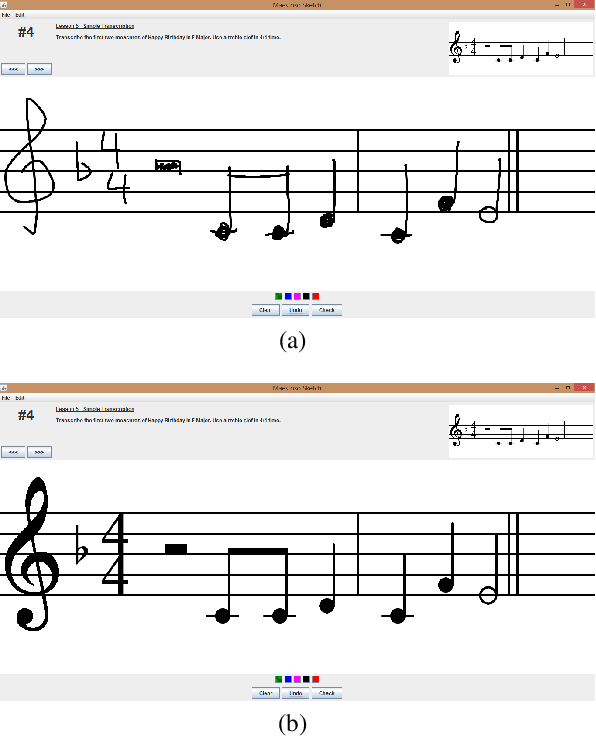
\includegraphics{images/maestoso.png}
   \caption{Maestoso Educational
   Sketching Tool for Learning Music Theory}
   \label{fig:taele2015maestoso}
\end{marginfigure}

The work of Taele et al. \cite{taele2015maestoso} \ref{fig:taele2015maestoso} describes the practical and cognitive benefits of learning music theory for both musicians and non-musicians. The paper proposes an intelligent educational tool to help students learn music theory. The tool, called Maestoso, utilizes sketch-based interaction and machine-learning techniques to provide personalized feedback to the user.
The paper first introduces the importance of music education and the challenges students face when learning music theory, such as the abstract nature of music concepts and the difficulty of translating musical ideas into notation.
Maestoso is a sketching interface that allows users to draw musical notes, chords, and melodies using a stylus or finger. The program uses machine learning algorithms to recognize the user's sketches and provide feedback on their accuracy and completeness.

\begin{marginfigure}
   \centering
   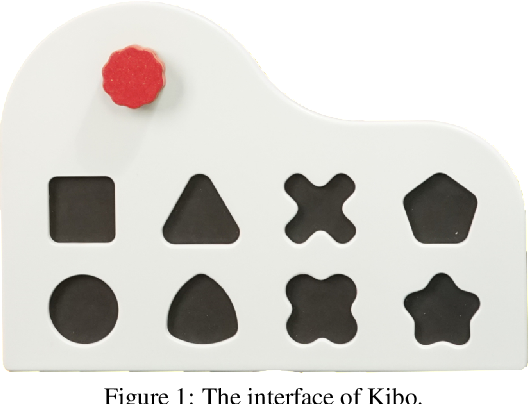
\includegraphics{images/IS_kibo.png}
   \caption{The interface of Kibo}
   \label{fig:amico2020kibo}
\end{marginfigure}

Amico et al. discuss the development of a new type of MIDI controller designed for music education \cite{amico2020kibo}. The device, called Kibo, is a tangible user interface that allows students to interact with music physically and intuitively.
The authors introduce the concept of tangible user interfaces and explain how they can be used to create more immersive and interactive learning experiences.
The device includes a set of modular blocks that the user can rearrange and customize to create different musical experiences.

Implementing such systems is often fully digital and interactive through a screen. Some projects aim to teach children music theory or interact with notes to compose, learn and experiment. Most of these projects are applications that users can download on smartphones or tablets. The relationship with the tangible paper score is gradually lost, and digital interaction replaces it more and more.

One solution is to use conductive ink to keep a tool in paper form without losing its interactive aspect. Conductive inks, paints, and varnishes are liquids containing metal particles, conductive polymers, or graphite. They have the specific ability to conduct electricity.

% TODO AJOUTER LES REFS AUX MARGINFIGURES

\begin{marginfigure}
   \centering
   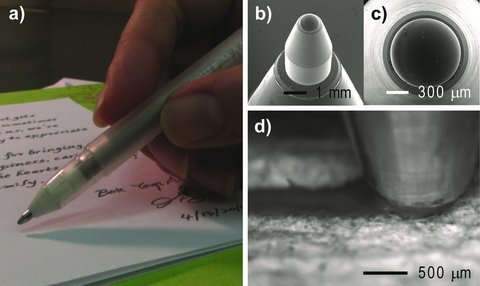
\includegraphics{images/IS_pen-on-paper.jpg}
   \caption{Pen-on-Paper Flexible Electronics. a) Optical image of a rollerball pen loaded with conductive silver ink. b) and c) side and top views of the rollerball pen. d) Optical image of the rollerball pen tip writing a conductive silver track}
   \label{fig:IS_pen-on-paper}
\end{marginfigure}

Inkjet printing allows to pattern of organic semiconductors \cite{kim2008heterogeneous}, metal contacts on organic semiconductors \cite{khan2019soft} \cite{wessely2020sprayable}, and metallic structures that require minimal further processing. Researchers such as Ahn et al. used conductive ink printing to realize metallic connections between functional components of flexible devices.



Another project like that of Russo et al. \cite{russo2011pen} has resulted in an optical image of a flexible paper display containing a LED array \ref{IS_pen-on-paper}. The prototype is a multi-color 25 × 16 LED array connected to the printed silver electrodes by depositing a drop of concentrated silver ink.

\section{General Architecture}

\subsection{Overview}




Our design augments a traditional paper score in many digital music learning applications on screen-based devices. Children already spend a considerable amount of time in front of screens, which can harm their eyes from a young age. Paper is flexible, lightweight, and easily transportable, and incorporating electronic circuits in the paper has shown its attractiveness to children \cite{hershman2018light}. 

\begin{figure}[h]
   \centering
   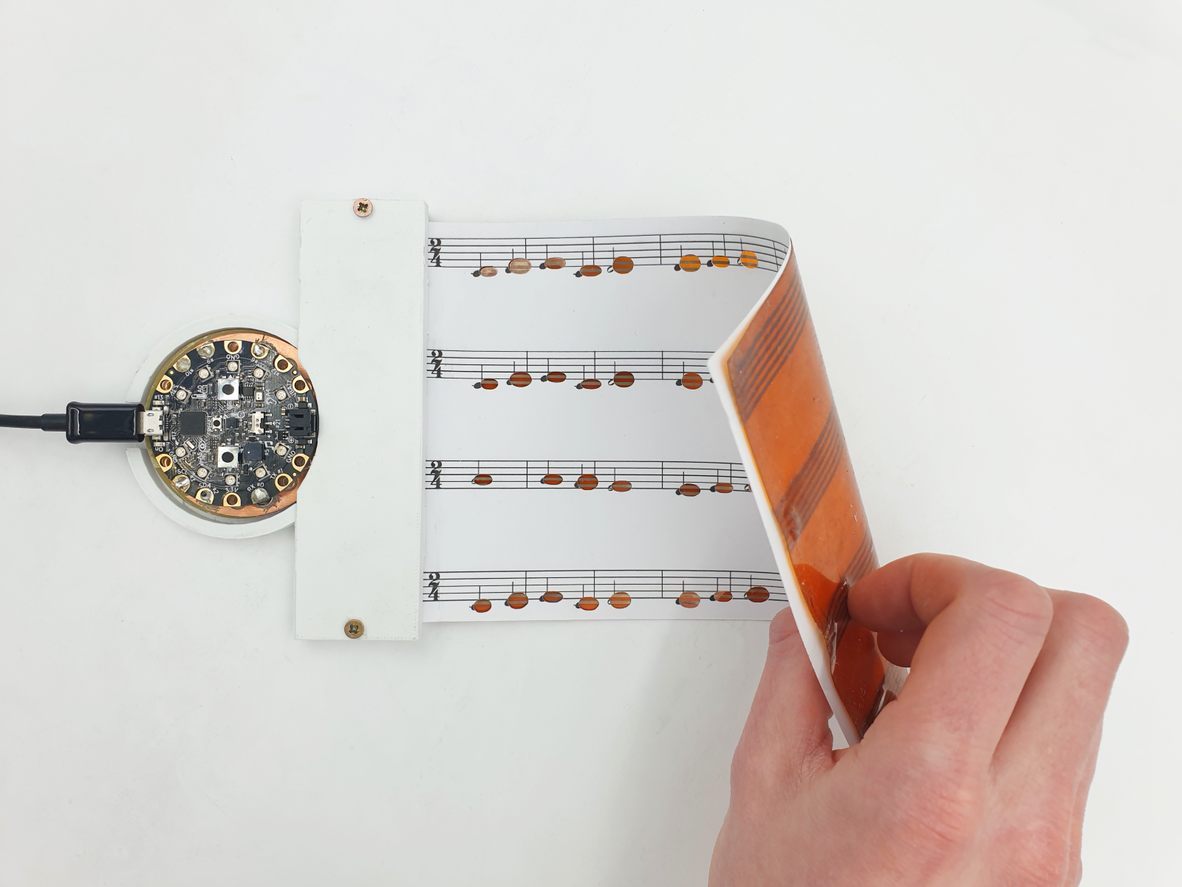
\includegraphics{images/IS_demo.png}
   \caption{Interactive Score Prototype}
   \label{fig:IS_demo}
\end{figure}

The project does not aim to teach a user how to play music. It seeks to link music theory directly with music practice without requiring knowledge.

The user has to supply the electronic part (substrate and PCB), then he places a partition (a cardboard stencil) on top of the substrate (where
the conductive lines are located) \ref{fig:IS_demo}. He can play the music and change it to another one.

\subsection{System Design}

The Interactive score consists of two thin layers. The first layer is the traditional sheet
music, printed on cardstock paper, with holes punched for each note. Under this sheet
is a polyimide substrate with conductive lines printed on it \ref{fig:IS_schema}.

\begin{figure}[h]
   \centering
   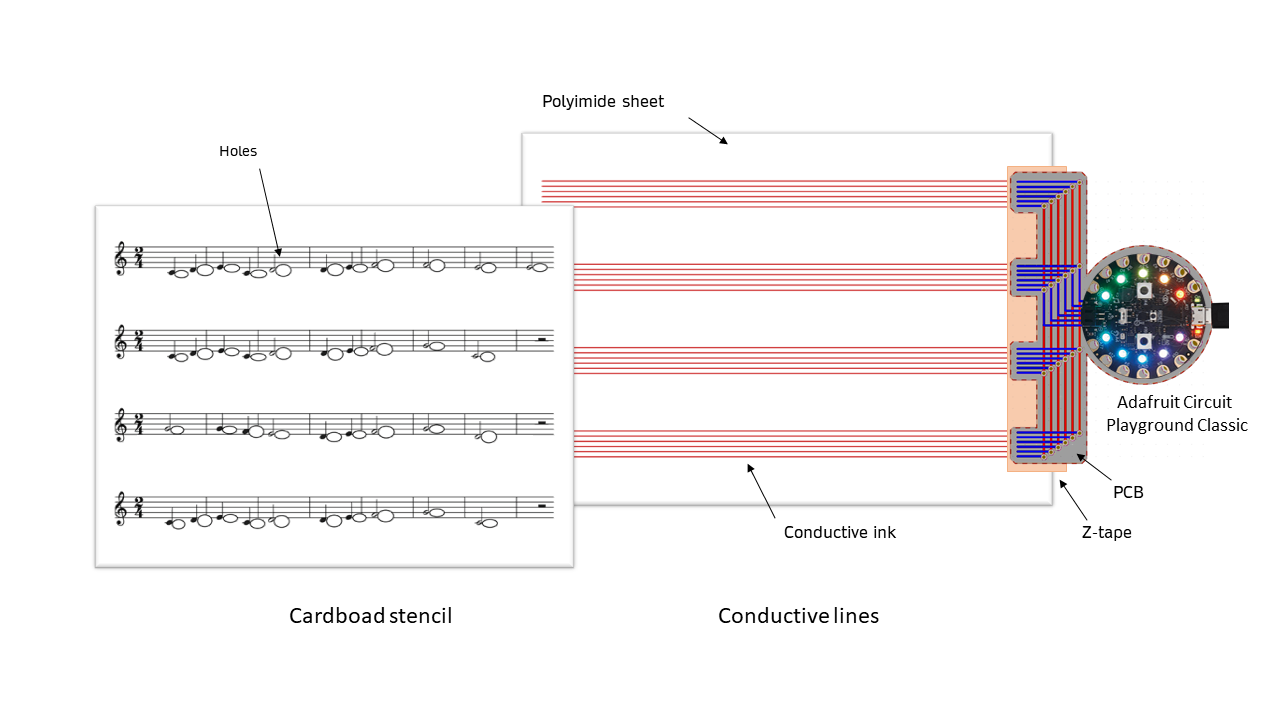
\includegraphics{images/IS_schema.png}
   \caption{Interactive Musical Score architecture.}
   \label{fig:IS_schema}
\end{figure}

The conductive lines are connected to an Adafruit Circuit Playground printed circuit board (PCB) using a double-sided "z-tape".

When the user touches a note on the top layer, the finger makes contact with the conductive lines through the holes in the cardstock.
The signal travels through the ink paths and the z-tape to the PCB, which detects a potential difference using capacitive touch and plays the relevant note. Detecting several simultaneous signals on multiple pins allows playing eleven different notes with only six lines \ref{fig:IS_schema}.

The system is kept in a 3D printed case, maintaining contact between the polyimide, the z tape, and the PCB. The user can easily open and close the case to change the music.



\subsection{Electronic Music Box}

The signal is recovered and used in capacitive touch with an Adafruit Circuit Playground Classic \ref{fig:circuit_playground_classic}. An Arduino program allows for generating a vast number of different notes. The code is retrievable on GitHub \cite{adrien2022capacitive_to_notes}.

\begin{marginfigure}
   \centering
   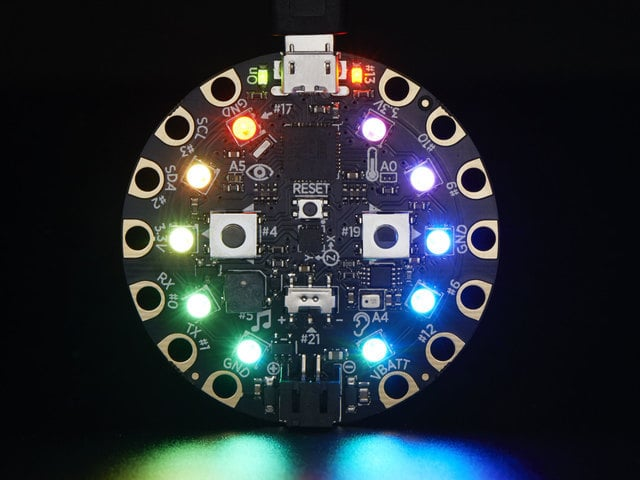
\includegraphics{images/circuit_playground_classic.jpg}
   \caption{Adafruit Circuit Playground Classic}
   \label{fig:circuit_playground_classic}
\end{marginfigure}

About the sound, the Adafruit Circuit Playground embarks a built-in buzzer. The implemented Mini Speaker is the SQMS5002S4036A. This device is a miniature magnetic speaker not adapted for playing detailed audio but for beeping, buzzing, and simple bleepy tunes. It is also possible to change the tone by changing the name of a variable in the code on the microcontroller.

The Adafruit circuit playground has ten mini NeoPixels of all colors, which can be animated with light when a user plays a note. The controller includes motion, temperature, light, sound sensors, a switch, and a mini speaker. This device is ideally suited for use on the score and integrates many features.

\subsection{Paper Score Manufacturing}

Notes, staves, lines, hyphenation, and cutouts were all placed on the same project for perfect dimensional compatibility between the different elements of the score. It allows the elements to fit together perfectly and export the cutout locations at the correct size relative to the partition's rest.

An inkjet printer draws all cardboard lines, hyphens, notes, and numbers.

A score of "J'ai du bon tabac" (on the left) lies on the substrate. Then, the notes were isolated in another PNG file, selected on Cricut design, and cut directly into the cardboard with Cricut maker 3.

% TODO Justifier les choix techniques

\subsection{Conductive Sheet Manufacturing}

The conductive ink paths are 1mm thick and 5cm long, with a resistance of 0.07 Ohms. A simple inkjet printer equipped to print with silver nanoparticles conductive ink drew the lines directly on the substrate. A hoven sintered the printed patterns at 180°C for 73 minutes. This process allows the quick production of flexible circuits \cite{khan2019soft}.

\begin{figure}[h]
   \centering
   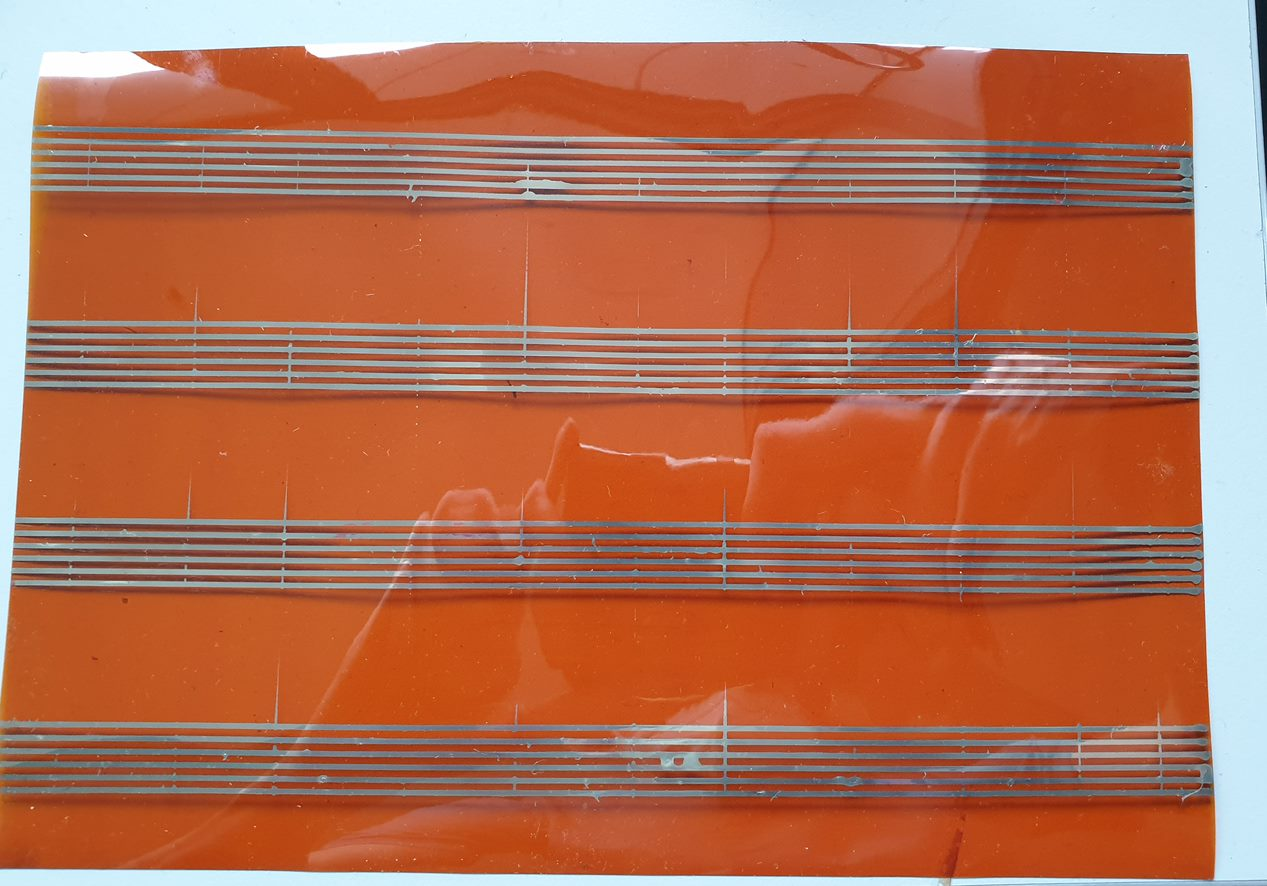
\includegraphics{images/IS_conductive_sheet.jpeg}
   \caption{Interactive Score Conductive Sheet}
   \label{fig:IS_conductive_sheet}
\end{figure}

This prototype comprises four staffs of 6 lines made of conductive ink on a Kapton polyimide sheet substrate. This polymer does not melt at high temperatures and has excellent mechanical strength, and is very dimensionally stable and creep resistant at temperatures above 260°C. The lines are 1mm thick, and at a distance of 15cm in length, it gave a resistance of 0.07 Ohms.

An Epson WF-2010 printer printed the lines on the substrate \cite{adrien2022capacitive_to_notes}.

Conductive ink allows the score to be flexible, like an actual musical score. The use of ink rather than flexible brass strips has the advantage of quickly printing interactive scores on an industrial scale. The material needed is only simple printers and ink and cleaning products for the printers. This process facilitates and accelerates production possibilities.

\subsection{Integration and Usability}

\subsubsection{Ability to change the score}

Its ease of interchangeability and production characterizes the paper score. The user can easily remove the paper sheet from the box and place another to play a different melody. All the electronic parts (substrate, PCB, microcontroller) are independent of the paper score. The sheet music has the exact dimensions of the substrate.
Therefore, placing the two precisely on each other to align the holes with the ink lines is simple.

\subsubsection{Ability to improvise}

The user can improvise by not playing the notes in the same order.
The project allows a great deal of modularity in its use. Just by touching specific notes at certain times, users can experiment with different rhythms and melodies and reconstruct a piece from a few notes.
With a simple score, including an ascending scale, he can try his hand at composition.
It is impossible to create dissonance as the Circuit Playground plays melodies in a fixed tonality set in the code. Unfortunately, this fact also limits the improvisation capacity.


\section{Applications and Evaluation}

\subsection{Set up}

Four users interact with the prototype already prepared for use. They then answer several questions. The project is plugged in and set up as a base for further use. Therefore, measuring the openness and visualization of music theory given by the project to the user is interesting. The questions concern understanding use, practicality, interest, innovation, attractiveness, and playfulness.

\subsection{Results}

The users did not encounter any particular problems during the test. The prototype worked well. The testers gave interesting feedback. The majority of the comments were positive, as the project considered most of their comments since a previous test.

The users proposed many ideas to make the project evolve. They advised adding indications, potentially with LEDs, to indicate actions to be carried out. One idea was to create a binder with different stencils inside. They would have appreciated a correction of the electronics, which would warn them if they made a mistake. The testers liked that the person playing has to press the right notes, unlike some music toys that automatically correct the sound to play the right notes wherever the user presses. The users were also very interested in the fact that the project is portable. They would have liked to be able to take it with them to play music everywhere.

\section{Discussion}

\subsection{Attractivity}

The project is attractive for children as a tangible object.
Its gamified aspect makes it close to a toy. This aspect contributes to its attractiveness, especially to young children. Its musical property favors the user's creativity in addition to being portable, tactile, fun, and easy to use.

\subsection{Musical Imagery learning}

An essential aspect of musical practice is the ability of the musician to decipher a score. When this one practices with visual support, his brain must take the exercise to connect the note, which he links visually with the position of his fingers on the instrument. The transcription of the note read is an intermediate the brain uses, deducing a position and calculating an interval from it. The ability to translate a visual note into a sound is a reflex to be trained and very relevant in the practice of music. The basics of this ability must be acquired very quickly when learning the basics of music.

\subsection{Mobilising multiple intelligences}

This kind of device has a genuine interest in terms of learning. The user practices bodily intelligence with touch, visual intelligence since he has a support in front of him, and musical-rhythmic intelligence.

\section{Conclusion}

In conclusion, the interactive score project has a bright future, as it implements a very recent technology to popularize it. This process could be industrialized and even replicable for individuals with some improvements and optimizations. In the future, our goal is to make the score more accessible. Features such as flexibility and a simple "plug and play" aspect make it attractive even to children.

\subsection{Limitations}

The project has some limitations being a prototype. The device is limited in terms of the number of playable notes. The conductive sheet has six lines of conductive ink, which allows for playing 13 different notes between C5 and F6. It is not possible to generate alterations while playing. This fact means that if the playground circuit is set in a specific key, it is impossible to play a note with an alteration not present in the score's framework. The key must also be changed manually at each score change (paper sheet).

The major problem of the prototype is in its transmission of electrical signals.
The most crucial problem of the project is its sensitivity to the electric field due to the use of capacitive touch. Near electric fields, the microcontroller can detect false contacts. The device must also be connected to a power outlet so that the potential difference calculated between the user's finger and the ground is remarkable. Otherwise, the playground circuit may not detect the touch of a line or start playing by itself because of the detection of surrounding electric fields. A user should therefore keep the device at a distance from electronic devices and metal surfaces.

Z-tape transmits the signal from the conductive sheet to the PCB (inside the box). This conductive tape can be damaged and cause false contacts after many uses and transport. The tape can not transmit the current to the lines, and some notes stop working.

Another problem is the conductive ink which can crumble, preventing the current from crossing certain lines. The ink traces are indeed quite fragile and easily damaged. The ink is only dried on the substrate, so its adhesion can weaken. As the user has to run his finger over the ink, he can also remove thin layers, thus causing some lines to break.

The prototype also presents a difficulty in overlaying the sheet paper on top of the polyimide sheet to align the notes with the ink lines while keeping a flexible system. The case was designed for this purpose but could be more effective.

The device also needs to be improved in terms of sound quality.
The speaker driver circuitry is an on/off transistor, so the device can only play square waves. The device's loudest frequency is around 4 KHz. The sound generated is shrill, very electronic, and of poor quality. It can thus slow down the desire to practice and does not resemble the sound of an instrument.

\subsection{Future works}

Adding the play of an alteration with three "buttons" usable thanks to the capacitive touch: flat, sharp, and natural, which the user can trigger with the index finger of the left hand, is an idea to answer the problem of changing the key. These buttons will allow the user to discover the notion of these three tools and their meaning. They would be an interesting tool that would add an improvisation capacity to the system.

A "musical tutorial" should be added so the user can listen to the score's music before playing it. The tutorial would allow the user to assimilate the musical rhythm (the time between playing each note) with the physical rhythm (the time between pressing notes).

The electronic PCB/microcontroller part should also be redesigned to no longer integrate an Adafruit Circuit Playground but a much smaller, handmade circuit. It would be possible to improve the speaker's quality and connect the device to Bluetooth or Wi-Fi to play music at a distance.
The next steps are also about looking for partnerships in children's education to research experimentations on the impact of this interactive score on music assimilation. Several parameters would be evaluated, such as concentration level, playing time, and knowledge retention. It is necessary to consider different strategies to transcript musical-rhythmic on this interactive score.

    \chapter{Sign Language Learning Game in AR}

\section{Introduction}

Sign Language is considered the main communication tool for deaf or hard of hearing people. It is a visual language that uses movements to provide people communication with the world. 

This sign language is too little used because it requires a significant investment to learn it and most people do not use it directly in their lives. SL is not understood by everyone, forming a communication gap between the mute and the able people. According to the World Health Organization (WHO) report, the number of people affected by hearing disability in 2020 was 466 million whose 34 million are children \cite{el2020sign}. Over 900 million people will have this disability by 2050.

In France in 2020, there were approximately 4 and 5 million deaf or hard of hearing people who have difficulties or are simply unable to communicate through speech. Concerning the deaf speakers of French Sign Language (LSF), the figures are uncertain: they oscillate between 80,000 and 120,000, depending on the sources.

In this work, we introduce a short video game to teach sign language. The application is intended to work on the DVIC Interactive Mirror but is fully functional on a simple PC.

This report deals with the implementation of an AI for sign language recognition (SLR) using the mediapipe framework in order to extract the user’s coordinates and to analyze them through a model in pytorch. The model is then implemented in a game engine to create a visual novel video game. The game is then adapted to an augmented mirror to allow the user to play it in augmented reality. The game stimulates the motivation of the player in order to favorise his learning.

\subsection{GOSAI for Augmented Mirroir}

GOSAI is a new framework to help the development of augmented interfaces on the computer with a display. This framework targets all developers, from beginners to experts. GOSAI offers
basic and often used augmented reality functionalities.

Its structure allows for components to be reused between
projects, thus building a general catalog of tools and
solutions that develops over time.

In addition, the framework uses mainstream programming languages to allow a wide range of developers to
use it. The framework is written in Python and Javascript.
Python is used for the framework’s core components,
while Javascript is used for display.

JavaScript is a flexible programming language. It is one of the core
technologies of web development, and everyone can use it on both the
front-end and the back-end.
It is a versatile and robust language for video game. The developers can use JavaScript to make games using a variety of platforms and tools. They can use both 2d and 3d libraries in combination with JavaScript to create fully-fledged games in the browser or external game engine platforms \cite{javascriptgaming}.

The following projects presented in this thesis are implemented on an augmented mirror running on the GOSAI software system.

The augmented mirror is a platform that provides extensive interaction between the real and the virtual world. The objective is to create a platform that can provide not only recreational use but also medical and educational use.

A one-way mirror is placed against a screen. The mirror reflects perfectly where the screen is black and can display  information when the pixels are emitting light. A camera is placed at the top of the mirror, facing slightly down.  A laptop is placed at the back of the screen.

The mirror can scan the room and detect and position objects the user interacts with. The augmented mirror uses the Intel D435 camera to estimate the position of a user in front of the mirror with Mediapipe. Thus, it can add a new dimension of interaction exploiting kinesthesia. This dimension is an advantage over traditional interfaces using touch or a mouse. 

This interface is ideal for the development of applications requiring movement. This is why it is relevant for the implementation of AI-assisted sign language learning modules.

\section{Related work}

\subsection{Sign Language Recognition}

A wide range of domains use SLR for different purposes. It can be found in robotics, human services, games, virtual reality applications, direct or remote communication or HCI projects \cite{adeyanju2021machine} \ref{fig:Polhemus}.

\begin{marginfigure}
    \centering
    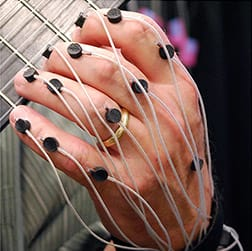
\includegraphics{AdrLfv_master_thesis/images/polhemus_tracker.jpg}
    \caption{Polhemus}
    \label{fig:Polhemus}
\end{marginfigure}

Many early SLR systems used data gloves and accelerometers to acquire specifics of the hands. The devices mesure x,y,z, orientation, velocity directly using a sensor such as the Polhemus tracker \cite{413199} \cite{5738842} or DataGlove \cite{Kadous1970} \cite{Metaxas1970} including accelerometers, gyroscopes, and electromyography sensors  \ref{fig:data_gloves}. Those techniques did not allow full natural movement and constricted the mobility of the signer, altering the signs performed and being restrictive because of the need of supplementary material.

\begin{marginfigure}
    \centering
    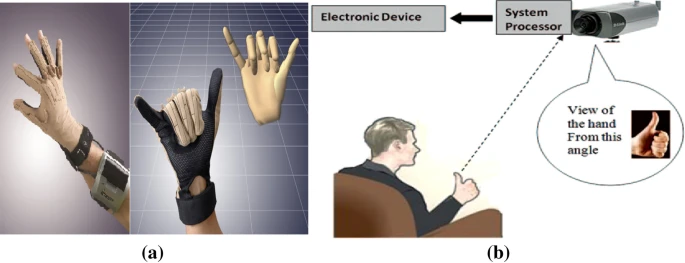
\includegraphics{AdrLfv_master_thesis/images/data_gloves.jpg}
    \caption{Human–computer interaction using: a CyberGlove-II \cite{cyberglovesystems}, b vision-based system}
    \label{fig:data_gloves}
\end{marginfigure}

Most techniques based on data gloves convert the position of fingers and hands according to their angles into electrical signals to obtain the desired sign. 

In 2010, the ImageNet files appeared \cite{li2010crowdsourcing}. They provided a basis for the CNNs and deep learning models used today. This was the beginning of computer vision. In 2012, AlexNet appeared and dramatically reduced the error rate for image recognition \cite{alom2018history}. After the appearance of these models, the use of data gloves is gradually abandoned to focus on the implementation of modules using computer vision.

Computer vision based techniques use pose estimation on the face, body, hands and fingers to detect their position. This method uses images or videos of the signs through the use of a camera and calculations on the images assisted by artificial intelligence \cite{adeyanju2021machine}. 

The identification of signs must take into account many different parameters. Facial expressions and body posture are key in determining the meaning of sentences, e.g. eyebrow position can determine the question type. Some signs are distinguishable only by lip shape, as they share a common manual sign \cite{cooper2011sign}. 


\begin{marginfigure}
    \centering
    
    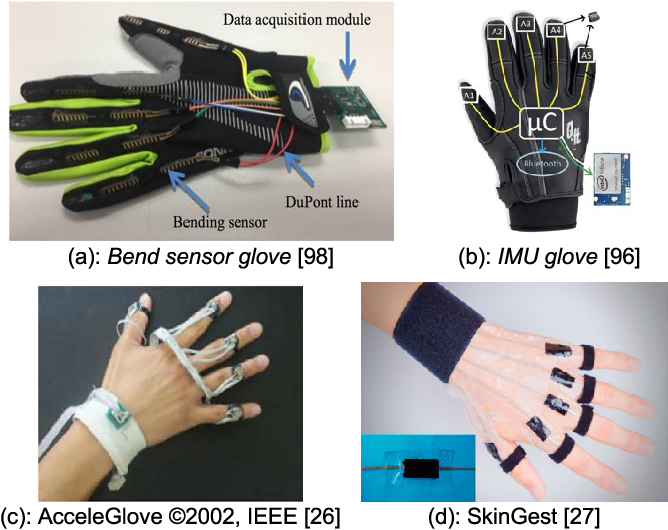
\includegraphics{AdrLfv_master_thesis/images/8-Figure2-1.png}
    \caption{Various custom gloves constructed by researchers in the sign language recognition field.}
    \label{fig:8-Figure2-1}
\end{marginfigure}

The speed of the sign realization can change the notion of speed induced by the performed sign. A sign can also depend on its position on the body. All limbs must therefore be taken into account during the analysis. These challenges include sensor placement, data collection and preprocessing, and model training and evaluation \cite{9178440} \ref{fig:8-Figure2-1}.

Sign language recognition systems based on computer vision and wearable sensors have been proposed by several researchers \cite{ionescu2005dynamic} \cite{yu2010vision} \cite{li2015feature} \cite{sonkusare2015review} \cite{bobic2016hand} \cite{islam2017real} \cite{islam2017real} \cite{saha2018machine}, \cite{rastgoo2021hand} \cite{xu2021application}. 

\begin{marginfigure}
    \centering
    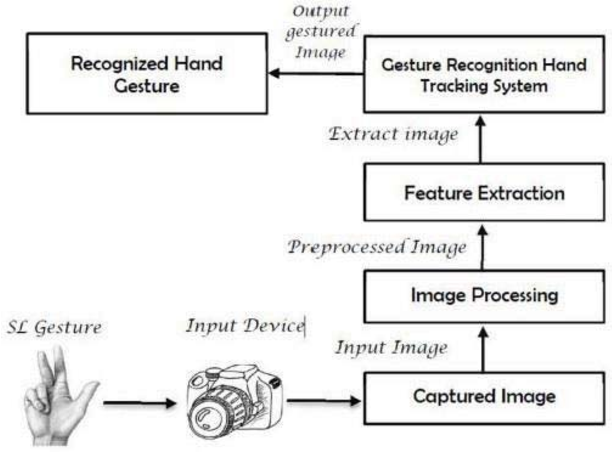
\includegraphics{AdrLfv_master_thesis/AdrLfv-main.tex/images/2-Figure2-1.png}
    \caption{Typical Vision Based Sign Language Recognition architecture.}
    \label{fig:2-Figure2-1}
\end{marginfigure}

Most recent SLR techniques use various image or vision based SLR systems comprising feature extraction and classification \cite{nimisha2020brief} \ref{fig:2-Figure2-1}. 

Many projects using computer vision assisted SLR exist \cite{admasu2010ethiopian} \cite{deriche2019intelligent} \cite{ahram2021advances} \cite{song2021intelligent} \cite{lee2021american} \cite{lee2021comparative} \cite{gao2021rnn}. 

A large part of these projects use a Convolutional Neural Network (CNN) model for predicting American Sign Language alphabet \cite{bin2019study}. Previously, different classifiers like support vector machine \cite{savur2015real}, random forest, multilayer perceptron, transfer learning, fine tuning \cite{saleh2020arabic} etc. have been introduced for sign language recognition on simple images. Recently, shallow CNN and Capsule Networks have obtained better results \cite{hasan2020classification}. 

Skeleton coordinate-based action recognition with coordinates has recently been attracting more and more attention to compute sign language videos because of its invariance to subject or background, whereas skeleton coordinate-based SLR only takes the data that is important for its learning. 

The most commonly used pose estimation frameworks that extract coordinates from a person using pose estimation are for example OpenPose \cite{cao2017realtime} \ref{1-Figure1-1}, MoveNet \cite{movenet}, PoseNet \cite{kendall2015posenet} and MediaPipe \cite{lugaresi2019mediapipe}.

\begin{marginfigure}
    \centering
    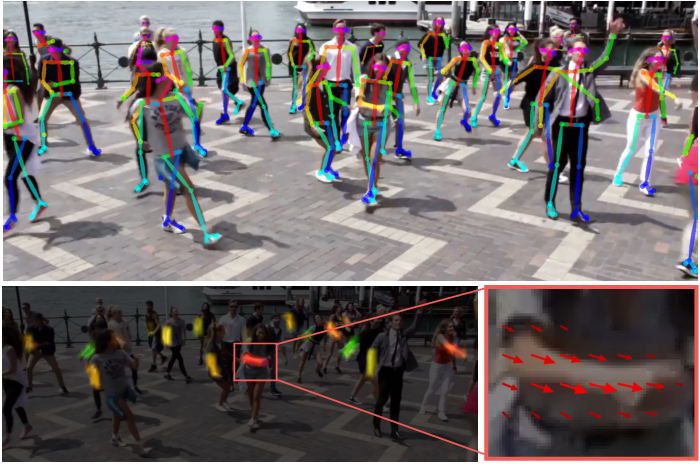
\includegraphics{AdrLfv_master_thesis/AdrLfv-main.tex/images/1-Figure1-1.png}
    \caption{Top: Multi-person pose estimation. Body parts belonging to the same person are linked, including foot keypoints (big toes, small toes, and heels). Bottom left: Part Affinity Fields (PAFs) corresponding to the limb connecting right elbow and wrist. The color encodes orientation. Bottom right: A 2D vector in each pixel of every PAF encodes the position and orientation of the limbs.}
    \label{fig:1-Figure1-1}
\end{marginfigure}

The recovered coordinates (extracted with computer vision or thanks to data gloves) are then processed with training methods. Various machine learning algorithms are then used for sign language recognition, including neural networks, support vector machines, and hidden Markov models \cite{9178440}.

Adeyanju et al. provides a comprehensive review of the state-of-the-art techniques used in sign language recognition using machine learning \cite{almeida2014feature} \ref{S0957417414003042}. The paper highlights the significance of sign language recognition and its potential to revolutionize the way communication is done between the deaf community and the hearing community. The authors then review the different machine learning techniques used for sign language recognition, such as Hidden Markov Models (HMMs), Support Vector Machines (SVMs), and Deep Neural Networks (DNNs).
The authors also highlight the importance of datasets in sign language recognition and review some of the commonly used datasets for sign language recognition. They emphasize the need for large, diverse datasets to train machine learning models effectively.

\begin{marginfigure}
    \centering
    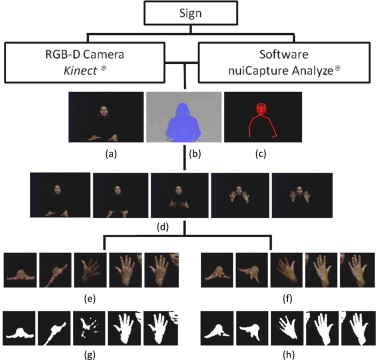
\includegraphics{AdrLfv_master_thesis/AdrLfv-main.tex/images/S0957417414003042.jpg}
    \caption{Feature extraction in Brazilian Sign Language Recognition based on phonological structure and using RGB-D sensors}
    \label{fig:S0957417414003042}
\end{marginfigure}

However, sign language is far more than just a collection of well specified gestures.

%TODO ajouter le concours de google

\subsection{Sign Language Learning Video Games}

The video game is a dynamic audiovisual entertainment platform, accessible and stimulating the imagination of players. There is a possibility of using them to strengthen skills and abilities within society. This is how video games are becoming a playful phenomenon, important in children's and youth culture.
Video games enhance the function of the attentional system, stimulate visual attention, reduce reaction time, improve the ability to discriminate shape and color, plus efficiency when following multiple object \cite{green2006enumeration}.

They are a good didactic way to promote interest and motivation by linking playfulness and pedagogical functions \cite{tejeiro2009efectos} .

The augmentation of interfaces thanks to technology causes a better attractiveness of the learning method and thus an increase of the time voluntarily dedicated to self-learning and of the motivation to concentrate on the method \cite{baker1994}.

Very few games use sign language as a basic element in the gameplay. We can cite Moss \cite{moss2018} \ref{moss-1200-80}, a video game on PlayStation VR in which the hero communicates with the player with ASL. 

\begin{marginfigure}
    \centering
    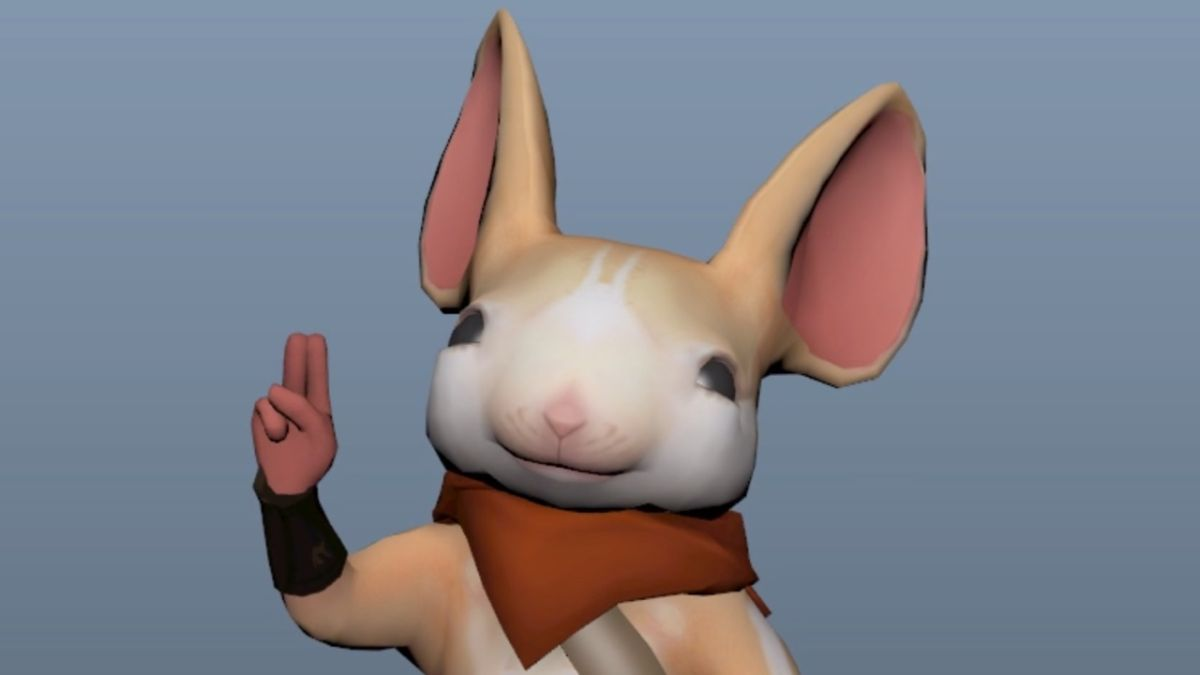
\includegraphics{AdrLfv_master_thesis/AdrLfv-main.tex/images/moss-1200-80.jpg}
    \caption{Moss hero communicating with the player through american sign language}
    \label{fig:moss-1200-80}
\end{marginfigure}

Zahoor Zafrulla et al. present Copycat, a game designed to improve the American Sign Language (ASL) skills of deaf children \cite{zafrulla2011copycat}. The game was developed by a team of researchers from the University of California in collaboration with members of the deaf community.
The game, called CopyCat, is a digital game that uses machine learning to provide feedback to the players. The game consists of a series of mini-games that focus on different aspects of ASL, such as finger spelling, vocabulary, and grammar \ref{aslgamecopycat}. In each mini-game, the player is presented with a video clip of a person signing a word or phrase in ASL. The player is then asked to copy the sign or phrase using their own signing.

\begin{marginfigure}
    \centering
    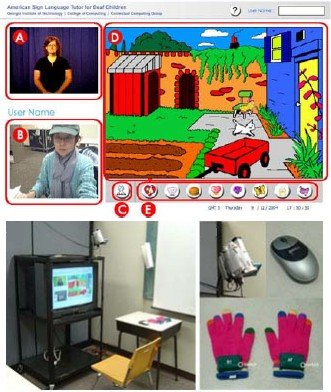
\includegraphics{AdrLfv_master_thesis/AdrLfv-main.tex/images/aslgamecopycat.jpeg}
    \caption{Screenshot of ASL Game Interface and the input devices for user  }
    \label{fig:aslgamecopycat}
\end{marginfigure}

CopyCat uses machine learning to analyze the player's signing and provide feedback on their performance. The game is designed to be adaptive, meaning that it adjusts the difficulty level based on the player's skill level. The game also tracks the player's progress and provides feedback on areas where they need improvement.
CopyCat developpers then enhanced their SLR system with the Kinect depth-mapping camera which uses colored gloves and embedded accelerometers to track children's hand movements \cite{zafrulla2011american}.

Bouzid et al. explore the use of a learning game for SignWriting, a system for writing sign languages, to enhance sign language learning for students \cite{bouzid2016using}. The game is designed to be played on a computer or tablet and includes a variety of activities such as matching signs to their written symbols and translating written symbols into signs.

Lesmes et al. discusses the development of educational video games for deaf children in order to facilitate their inclusion in mainstream educational settings \cite{lesmes2022design}. The paper outlines the design and development process of educational video games, including the use of a participatory design approach that involved deaf children and educators throughout the design process. The games were designed to incorporate sign language, visual cues, and other features that would make them accessible to deaf children.

Many applications on smartphones aim at learning sign language. Some target children by displaying animals demonstrated in 3D (SignEveil).
Most of these applications are in a quiz with a lesson part and a questionnaire part. It is not possible to interact by making the signs yourself.
JavaScript is used extensively in games that do not require many resources. A 2D interactive game displays only a few details and elements.

JavaScript is a language adapted for such a creation. Frameworks like Phaser JS library or simply P5 are suitable for coding a small game. p5.js is a JavaScript library for creative coding, focusing on making coding accessible and inclusive for artists, designers, educators, beginners, and anyone else. It can display graphics and process many different elements.

% Parler de pocket sign

\subsection{Visual Novel Engines}

P5VN is an open-source Interactive Design and Media Major at NYU Tandon School of Engineering student project, allowing to create a visual novel using P5.js. It allows to display dialogues, sprites, as well as backgrounds and use menus by clicking. The game scenario is easily editable through a script, which is then parsed by the engine. The original aim of the project was to implement a prototype engine based in p5.js with a custom scripting language.  

Other visual novel engine, Tuesday JS \cite{TuesdayJS} or Monogatari \cite{monogatari} are simple web-based visual novel editor that can be used in a web browser. They are written in JavaScript allowing the use of vector graphics svg, gif animations and css styles.

Tuesay.js is an easy to use visual novel editor. Free and open source, it runs on any web browser. It is written in JavaScript, does not use third-party libraries and therefore does not require additional software installation. It uses a drag-and-drop interface for editing scenes and creating interfaces. The script is displayed as a flowchart with all the elements and branches of the plot. This makes it easy to navigate and helps you create stories with many plot options.

Monogatari.io is similar to Tuesday.js. The platform support different medias (images, videos, music), multiple languages. It is highly customizable, open source and multi-platform. 

\subsection{Animated 3D Avatar}

For the creation of an animated avatar, most systems implement the display of an animated model from an animation software (Blender, 3DS Max, Maya, Unity, Houdini...). The animations are worked directly in the software and then imported into a program for display in a game. 
Some projects allow the animation of a 3D model directly from the motion capture. In the project "Real-time Avatar Animation from a Single Image" \cite{saragih2011real} Saragih et Al. realize the modeling of 3D models from a simple photograph \cite{saragih2011real}. 

A tool such as Unity or Maya can make its animation from MediaPipe coordinates. A tool that gives nice rendering for 2D animation is Pose Animator. A demonstration works with FaceMesh and PoseNet (from MediaPipe) online \cite{pose\_animator}. Unfortunately, this one does not understand finger movements. Adapting this system to MediaPipe by adding finger movements can give a free 2D avatar. 

Another way is to adapt the coordinates in real-time to animate a character on Blender using Daz Studio as Nguyen et Al. \cite{nguyen2021automatic}.
Many other demos of characters built with MediaPipe exist. Most use MediaPipe and TensorFlow.js (namely FaceMesh, BlazePose and HandPose) \cite{blazepose}.

Another project allows moving a 3D model with Three.js (React Three Fiber) and Tensorflow’s Pose Estimation model (PoseNet). The model uses Tensorflow and PoseNet to detect the key points of the joints in each frame and then send those points over to the Model file. The project uses an Adobe Mixamo 3D model in FBX format and Blender to import the FBX format and export a GLB format \cite{posenet}.

A last interesting example is that of Kalidokit \cite{kalidokit}. Kalidokit is a tool that uses Mediapipe/Tensorflow.js models for tracking face, eyes, pose, and hand movements. It is compatible with various models such as Facemesh, Blazepose, Handpose, and Holistic. The tool calculates simple euler rotations and blendshape face values based on the predicted 3D landmarks.

Kalidokit is the core component for Vtuber web apps, such as Kalidoface and Kalidoface 3D. Its purpose is to rig 3D VRM models and Live2D avatars. The project is a JS library intended for developers using Mediapipe pretrained models and not a complete app on its own. The library still has to be adapted to run on different platforms. The project is based on Three.js, a powerful library for creating three-dimensional models and games. 
With just a few lines of JavaScript, it allows the creation of simple 3D patterns to photorealistic, real-time scenes. The library can create complex 3D geometrics, and animate and move objects.

Three.js enables the application of textures and materials. It also provides various light sources to illuminate scenes, advanced postprocessing effects, custom shaders, load objects from 3D modeling software... It is easy to use, intuitive, and a well-documented library.

\section{Gameplay}

The sign language game is an augmented reality game, a visual novel on the augmented mirror. We follow a character during a short adventure in which the user can take choices by making American Sign Language signs in front of the mirror. He can answer to the characters, interact with objects, choose actions and choose a path. 
Sometimes the player sees the tutorial of one, two, or three signs at the same time. The user must then make the sign of the choice he takes. For example he can choose to turn right or left by making the appropriate sign. 
3D avatars are the models for all the characters. Their limbs (including fingers) are animated. Only the character Aria (the hero's friend) is performing the sign tutorials.
The signs made are detected by the camera and guessed by an AI working in back end. Dialogue lines appear during the adventure to guide and discuss with the player. The user must make the "ok" sign with his hand to scroll the text.


\section{General Architecture}

\subsection{Visual Novel Engine}

\subsubsection{Engine implementation}

The best solution to make such a game was the implementation of a visual novel engine on the mirror from which to develop everything else in the game. P5VN engine is precisely  basically adaptable for the mirror because the engine is basically working with p5.js.

Previouly, p5VN was able to load and display background, sprites of characters, some text interactive with the mouse click, menus with multiple buttons for the user to take choices.
The engine was running synchronously in a single thread.
After an important adaption. The module is now running asynchronously to be compatible with gosai. 
The engine now loads and plays video animations automaticaly at launch, the user can now interact and select menus thanks to sign language and added many other features.

\subsubsection{Menu}

In a visual novel, the player does not interact directly with the keyboard but must click on menu buttons to make choices. As the user interacts with the mirror only by the estimated pose, the menu system had to be adapted to both enable debugging by clicking and making choices with movements.

Each time a menu appears, it takes the form of three words aligned and distributed horizontally on the screen. An avatar of Aria appears behind each word to demonstrate the sign related to this word. The location of the words and the 3D tutorials are spread over the width of the screen according to the number of buttons in the displayed menu. 

Aria's avatar animation plays in a loop until the player makes a sign detected by the SLR module and included in the menu. The path taken by the game is then directed towards the continuity of the chosen branch.

\subsubsection{Script}

The game script is contained in a script.txt file in the application components. It contains a set of commands starting with the \$ symbol telling the game to do a particular action. These commands can be :
\$tag which indicates a specific point in the script
\$jump to jump to a tag
\$defineC to define a character (name, sprite address, text color)
\$defineImg to define an image
\$bg to display a background
\$show to display a character
\$addAnimation to play an animation to a character
\$setSprite to display the sprite of a character
\$menu to create a new menu
\$hide to hide a character
\$setvar to set a variable to a value
\$if to manage if then else commands

All the loading of sprites, animations, their playback, display is now managed automatically at startup in asynchronous instead of being set manually in the script or in the code as before. The engine running in synchronous mode at the beginning, a sprite could not be called before being loaded. The game starts on a loading time at startup corresponding to the loading of sprites and animation videos in the memory of gosai. This allows each animation to be played instantly when each one is called.

\subsection{Animations}

The most efficient way to create accurate custom 3D animations for the animated sign language tutorials was to implement a module allowing to control an avatar in 3D through pose estimation and then record the movements produced or a video of the animation.

An application to control an avatar remotely thanks to the estimation pose has been developed on the augmented mirror. The avatar is able to track and copy accurately the position of the user's limbs. The created application is now in free demonstration on the mirror. It also allowed to create all the 3D character animations on the sign language learning game.

\subsubsection{Esla}

The Educative Sign Language Avatar (ESLA) is a 3-dimensional avatar controllable in a gosai application following the estimated MediaPipe pose. Its movements copy live those of the user in front of the mirror \cite{esla}. It was the first version of the interactive avatar on the augmented mirror.

An animated 3D character appears on top of the scenery at the launch of the application. Its animation is made possible by playing features using MediaPipe and OpenCV. The program can retrieve the coordinates of a user’s position in real time. These coordinates are processed, and the avatar copies the movements Animation Retargeting, a video game animation technique using motion capture.

The programs retrieves the links between each point of the pose provided by MediaPipe and Three.js calculates and display the 3D part. 

Three.js entirely manage the loading of the character, its display, its animation, the rendering, the light and the camera .

Three.js uses a pivot system with matrix4 and quaternions. However, some functions to transfer rotations from one base to
another are missing (even though they are very much in demand by the community). Therefore, the entire limb rotation system was implemented by hand.
MediaPipe first retrieves the (real) coordinates of the user. These coordinates are converted into the world base (x-axis to the right, y-axis to the top, z-axis to the camera) of the three.js scene with transformations. The program retrieves the coordinates of the top of the spine, the shoulder, and the elbow. It creates two vectors spine/shoulder and shoulder/elbow. The coordinates of these two vectors are then read from the base of the parent of the bone to be rotated (here the left shoulder). An algorithm then calculates a quaternion containing the rotation data from the first vector to the second.

This quaternion is then applied to the limb, which takes in its local base the same rotation as the user’s arm with his shoulder.
This allows you to make precise rotation transfers from one base to another and thus animate all parts of the avatar.

Unfortunately, the project lacks a lot of precision in the movements, especially at the level of the fingers, which is very inconvenient for the creation of accurate tutorials in sign language. Another more efficient solution for the creation of 3D animations with the estimated pose had to be implemented.

\subsubsection{Kalidokit module implementation}

The most important part of making the 3D animations the management of the avatar from Mediapipe, it is enabled by the Kalidokit solver. This JS library allowing the animation of arms, hands, fingers, face, mouth, eyelids, pupil of VRM models (Virtual Reality Model). The VRM is formulated on the basis of the standard 3D format glTF2.0 to manage humanoid models. It aims to be particularly expressive. This type of model has a large number of articulations, can blink and animate its mouth. It is very often used in the world of VR games (VR chat for example), or by Vtubers (entertainment broadcasters who use a virtual avatar).  

The models used are downloaded from the site Vroid Hub cite\cite{vroid}. They must respect specific conditions of use: use by a third party, downloadable, use as an avatar, commercial use by a company. The avatar must also be sober. The one that has been selected to be implemented in the demo application allowing to control the avatar in augmented reality on the mirror is called "papa\_de\_him\_chan". 

The model is easily changeable locally in the application created to allow the user to manipulate different characters. It is with this application that will be created the animations of tutorials of sign language for the learning game on the mirror.

Such an application therefore allows to record qualitative signs and poses for the characters and tutorials of the game.

The models used for the characters of Aria, the grandmother and the salesman were recovered on Vroid Hub and are free to use. The VRM models are mainly adapted for Vtubers, that's why the characters can look very childish and like Japanese anime characters.

\section{Sign Language AI}

\subsection{Overview}

Sign language involves the usage of the upper part of the body, such as hand gestures, facial expression, lip-reading, head nodding and body postures to disseminate information \cite{adeyanju2021machine}.

The final goal of this work is to implement an SLR AI inside the sign language learning game. This AI allows the recognition of choices in the game thanks to the esimation of the user's pose but also the control of the game using commands linked to signs.

Many models with sign language recognition already exist. The work done here proposes a model, as well as an easy system of creation, dataset management, training and visualization of the data.

\subsection{Integration in Gosai}

The project of creating the SLR AI is apart from gosai \cite{slr\_mirror}. Only the weights are integrated in gosai in a module making the comparison between a sign made in front of the camera and the values of the weights recorded locally.

The video game retrieves the coordinates of the user and place them in tensors containing the data of a video of 30 frames.

The model is called by passing the data to it and a table of probabilities concerning each action is retrieved as a result. 

The guessed sign is then transmitted from the slr module through gosai’s redis database to the game engine. When the probability of a detected sign overfits a threshold, the sign is considered as validated by the game engine.

\subsection{Structure}

The project is divided into 6 different local modules and a main file that initializes the parameters and launches the different processes. The processes are an optional phase of dataset creation, a tutorial phase that displays the skeleton for data vizualisation, a preprocess phase that retrieves the data from the dataset and formats them, a data augmentation module, and a weight calculation and exportation in different file types.

\paragraph{Dataset}

If a movement is included in the known actions but is not found in the files, the creation of the dataset of this movement is launched automatically. 

The dataset is created by the user and stored in a folder "MP data" created, and separated in three
folders : train, valid, test containing the actions (name of the
movement). The recorded sequences are automatically separated
between the three folders train (80\% of them), test (10\%) and valid
(10\%). Each sequence is 30 frames each by default, including coordinates, that is to say and now 116 data per frame (that is to say 58 points) after having removed  431 points of the face and just Keeping 4. The 4 kept points are one for the chin, for the forehead, for the wright and left cheek.
It enables signs using the head to be better detected.

The coordinates are retrieved from Mediapipe during the creation of the dataset. The recording is done from the webcam of the device used, an intel real sense or the default pc webcam if the intel is not detected. When implementing on another device such as the interractive mirror, this driver must be modified to match that of the camera used.

At the start of the dataset creation, the user alternates one second of video recording, then two seconds to reposition in a loop for each sign. He has a video feedback on himself to check if he is well positioned in the plan.

\paragraph{The recorded signs visualisation}

The recorded signs visualisation module (data\_vis) retrieves the coordinates of a video by action, stored in the dataset.
It sorts the coordinates of the points of each part of the body,
finds the different links between each point and the posters, frame
by frame. Arrays of all the sorted coordinates for each body
part (Face if activated, Body, Hand) are used, as well as all the links
of the body arrays.

For each point detected in the dataset, the visualization displays the links it has with the points it is linked to in the table. The program also display the action to which the visualization is associated, above the drawn character.

\paragraph{Preprocess}

The preprocess phase retrieves all the data from the dataset and places them in tensors to provide them to the model.
After creating the preprocess instances (according to their type: train, test, valid) we pass them to the dataloader. 

These pass an index to them (concerning a sequence among all the sequences attributed to the type of the preprocess). Their program calculates which action is concerned by the desired sequence and recovers all the coordinates of the frames of this sequence. 
In some papers, it is said that some sign language movements are only possible by giving some indications with lips or facial expressions \cite{cooper2011sign}. Some of the lip coordinates should therefore be kept in the dataset retrieval during the preprocess. For other papers, it is just not necessary to keep these points which take a lot of storage for nothing \cite{dreuw2007speech}.

The preprocess does not use all the coordinates of the face, this allows to have much faster train loops because all these points are not necessary.

\paragraph{Data augmentation}

The data augmentation is called during the pre-processing phase,
just after retrieving the data of the concerned sequence. It is given
the data as a parameter, it reviews the data and will apply a random
horizontal and vertical shift and scale to it. This process artificially
increases the number of positions in which the user can stand.

\paragraph{Model}

The model is composed of a bidirectional LTSM, a linear, a dropout, a batchnorm1d, a relu, and an other Linear. The AI trained on 16 different signs or 1600 sequences. The model reaches an accuracy of 87\% on the test set and 96\% on the training.

Recurrent Neural Networks (RNN) allow to process temporal sequences (language, videos, numerical data). They keep the memory of past data to predict data sequences in the near future. This is why LSTM and Bidirectional layers are used into the model. The LSTM (Long-Short-Term-Memory) are composed of several gates (respectively 3 and 2) which allow to forget or to selectively memorize the information of the previous temporal sequence in a dynamic memory.
LSTMs have an internal memory that is constantly changing dynamically according to the input data sequences.

The training uses the optimizer AdamW, a stochastic gradient descent method that is based on adaptive estimation of first-order and second-order moments with an added method to decay weights \cite{loshchilov2017decoupled}. 

Models are automatically exported in pth format, a common PyTorch convention is to save models. They can also be exported to onnx (Open Neural Network Exchange) \cite{onnx}, an open format designed to represent machine learning models. This extension enables greater interoperability in the AI tool community, allowing a large number of AI frameworks to be more compatible by allowing them to share models. This interoperability allows trained models to be easily deployed in different software platforms like GOSAI.

The onnx models retrieved from the project output are then directly implemented in the SLR module of gosai.

%TODO Ajouter une image des résultats

\subsection{Configuration}

All the processes mentioned above are optional. This management is located in a config.json file in which the user can enable or disable a large number of project features. 

All the options are : "actions" (all the signs recognized by the AI, "adapt\_for\_mirror" (to transform the coordinates specificaly for the augmented mirror),"convert\_files" (to convert the files from pth to onnx), "erase\_dataset" (to erase the dataset before recording a new one, by default the program automaticaly completes the existing dataset), "erase\_runs" (erase the local tensorboard files), "make\_data\_augmentation", "make\_dataset", "make\_train", "make\_tuto"  (visualization of the recorded movements), "nb\_epochs", "nb\_sequences" (total video number the user wants to record for a sign), "sequence\_length" (one video frame number).

The default actions are "nothing", "empty", "ok", "yes", "no", "left", "right", "house", "store", "hello", "goodbye", "television", "leave", "eat", "apple", and "peach". Those are all the signs used inside the SL video game.

The project aims for making it as easy as possible for the user to create weights according to his desired characteristics.

% ajouter schéma du modele
% parler de la visualisation des résultats

\subsection{Visualization of the results}

TensorBoard is a tool providing visualization solutions to machine learning tests. It allows to track and visualize metrics such as loss and correctness. TensorBoard allows displaying the graph of the exported model, displaying histograms of weights, biases or other Tensors, and many other functions.

Just by entering the "make set-up\_tensorboard" function in the terminal (or by doing a "make first\_boot"), the user launches the creation of a local server running on port 6006, retrieving the weights as the model is trained. 

A browser page then opens automatically to access the local server address. On this page the user can study a graph of the training and test phase (percentage of success according to the number of epochs). 

The logs of these results are stored locally, they are accessible and can be easily compared between them. This makes experimentation easier and more intuitive.

\subsection{Limitations}

After many experiments, several biases have appeared that directly affect the AI results. For example, the size of a user differing too much from the person who created the dataset is sometimes problematic, resulting in a strong difference in recognition performance between users with the same or different morphology. 

Since the AI bases its training on the data obtained from Mediapipe, the results of the SLR also depend on its parameters. It was observed that Mediapipe was better at recognizing the limbs of a person with a strong contrast with the background. 

This resulted in a very significant difference of about 15\% in performance on the training and test set. When the dataset was created by a person wearing a black shirt, his white skin was better detected by Mediapipe and better recognized afterwards. 

The same thing happened when using the sign recognition directly, with a t-shirt allowing a better contrast, the recognition was only favored. This also causes the fact that signs made on the belly (being a plain background without detail) are much better recognized than those made on other places with more potential details in the background.

\section{Usage scenario}

The augmented mirror is primarily aimed at families and is designed to be placed in a living room. Its use is very wide and allows to have fun as well as to learn by interacting.
The mirror does not require any additional material, so its use remains very simple.
The learning game of the sign language is directly launched from the menu of the mirror. The user just has to follow the instructions given by Aria to follow the course of the adventure. The game is primarily aimed at young children. Through repetition and distraction, they intuitively learn certain gestures.

\section{User study}

\subsection{Set Up}

As the sign language learning game is intended for young users, this test focuses on a sample of 12 people between 18 and 25 years old.
6 people watch a number of video sign language tutorials on the "pocket sign" application. The signs viewed correspond to those encountered in the game when choosing the path through the house ("ok", "yes", "left", "right", "house", "store", "hello", "goodbye", "television", "leave", "eat") or the path through the store ("ok", "yes", "no", "left", "right", "house", "store", "goodbye", "apple", "peach"). 4 people view the signs of the passage through the house and 2 view the signs of the passage through the store.
When they think they have understood the sign viewed, they skip to the next sign. 

6 other people use the sign language learning game on the mirror. They are told the principle of the game before using it. Two of them go through the house and four of them go through the store.

Both groups are told at the beginning that they will be evaluated on certain signs at the end of the study. 
For both groups, the session is timed from start to finish.

\subsection{Results}

\paragraph{Sign Language Video Game}

In one session, users took an average of 4.44 seconds from game launch to completion. Some users have experienced problems related to poor AI recognition.
Notably for the sign "peach" and the sign "eat" difficult for two users.

One user took 8:25 to complete the game. He had great difficulty in making the "go" sign in the house. This bias is explained by the fact that the dataset was created by a tall person (1,84m) and this user had a much smaller height (1,60m). 

Users were tested after their session on some random signs. Their average score was 2.33 signs learned out of 4. The errors made are related to several elements. The AI sometimes finds a sign far too quickly when the user has not yet placed his hands correctly. The user then has no time to look at the signs and make his choice. Another error is related to the fact that when there are three tutorials at the same time (menus with three choices), the user has more difficulty to concentrate on each one and his memorization of the signs is less efficient.

To correct the problem related to the too high detection speed of the AI, increasing the detection treshold value would be an efficient method.

To conclude, people were asked to note on 10 their opinion about diverse questions. Their average motivation to learn sign language in this particular way (with an augmented mirror and the video game) was 7,91/10.
The average fun in interacting notation was 8,25/10. Their ease of understanding what needs to be done had a notation 7,58/10. The practicality of using this learning method (augmented mirror) had a notation of 8,25/10.The effectivity of using this learning method received a notation of 6,41/10. And the capacity of the AI to guess the correct sign was noted 6,11/10.

The global feedbacks were that the avatar sometimes moves his fingers too much and could not be very precise. The fact that the display is in 2D (on the mirror screen) and not in 3D makes it difficult to understand the signs.
One user was blocked by the fact that the characters look like anime characters and not more realistic ones, which can put off the desire to practice.
Some users forgot the "ok" sign to skip dialogues during the game although the sign was shown twice at the beginning of the game. This prevented them from continuing the practice without external intervention to remind them of the sign. 
One user had learning difficulties due to the avatar's movements being considered unclear. Interacting with a real person, however, allowed him to learn more effectively. The lack of accuracy of the AI was also strongly criticized (rated 6.11/10 by users). This accuracy is almost perfect for the creator of the dataset, but low to other users with a different morphology.

The 3D animated tutorials were generally liked and were considered more attractive than simple video tutorials. The fact that the game was implemented on an augmented mirror was praised because this interface is considered to be mainstream and easy to integrate in a living room.


\paragraph{Videos}

%TODO implémenter la seconde partie de la user study 

\section{Discussions}

The SL Game stimulates the visual, verbal and kinesthetic intelligence. 

The visual intelligence is the ability to create mental images, and to perceive the visible world with precision in its three dimensions. Viewing 3D sign language tutorials and having to "decode" the different movements and positions of the avatars' limbs stimulate the user's visual intelligence. The user needs to perceive, to make a mental projection before re-performing the identified signs.

Verbal intelligence is the ability to read, speak easily and connect mental ideas into words. Having to connect a picture to a word in the project leads to the ability to express oneself fluently and therefore to connect the mental idea of a word into a gesture. 

Kinesthetic intelligence is the ability to use one's body in a fine and elaborate way, to express oneself through movement, to control one's body movements well. This type of intelligence is stimulated through play in this project because the brain must translate the mental image of body positions and movements in space into real positions and movements. 

The stimulation of three different intelligences, added to the motivating gamification aspect, favors information retention. The user can remember a particular gesture by the memory of having seen it and projected it mentally, by the memory of having given it a linguistic meaning, and by the memory of having performed it physically in space.

\section{Conclusion}

\subsection{Playful Learning and ASL}

Playful learning and gamification are learning methods that use playful elements to facilitate the assimilation of knowledge. 

Learning video games are a popular form of these approaches and are often used to teach practical skills such as sign language. The use of augmented reality, pose estimation, and artificial intelligence in the Sign Language Video Game creates an immersive and interactive experience for the learner to practice reproducing signs correctly in real time. This approach promotes learning by providing instant feedback and allowing the learner to practice as many times as they want. 

In addition, the use of cutting-edge technology often generates interest and engagement in the learner, which can help to increase motivation and perseverance in learning sign language.

\subsection{Limitations}

The results of the user studies make it possible to extract a certain number of limitations from the project.

The size difference between the person who created the dataset and a potentially taller or shorter user is problematic. This can be solved by applying a compression of the coordinates to the horizontal and vertical axis randomly in the data augmentation or by registering the dataset by people of different sizes.

The dataset produced and used is small. It contains little noise, little variation, and little mixing. The model is also moderately efficient and could be reworked especially with the use of transformers. The model is also trained on few different signs (15). This means that in the case of an enlargement of the dataset, the accuracy would tend to decrease even more. It is therefore necessary that the model and the dataset be reworked in the future.

Another important limitation is the sometimes difficult clarity of avatars in sign language tutorials. The pivot angles of each of the avatar's bones being limited to avoid glitches and ragdolls, it is sometimes hard to record precise signs especially at the finger level. The user must then imitate and learn a model that is not totally accurate. The avatar can be slightly reworked to widen the achievable angles and thus gain in precision.

\subsection{Future Works}

The current system is good for direct practice but too easy because users can afford to just copy the sign. It would be necessary to add an evaluation dimension with signs that come up in the potential choices without giving the tutorials every time. Thus the user will have to force himself to remember and will have a better learning by repetition.

This work has already been done in another application on the mirror similar to a sign language training. The application consists of successive viewings of sign language tutorial videos, practice, and finally correction. 

The correction phase consists of a frozen Mediapipe skeleton appearing on the mirror and performing the beginning of a sign (first frame of a recorded movement). 

The user also has a Mediapipe skeleton displayed on the mirror and following his position. When he superimposes his own skeleton on that of the model, the model's skeleton moves slightly to display the next frame. 

The user must then superimpose his skeleton on the second frame and so on until he has validated the 30 frames that make up a sign. The person must superimpose some points of his body, but especially his hands and in particular his fingers. This allows him to learn with precision the sign he has just made. The training then moves to a tutorial of another sign. 

The implementation of the correction phase of this training in the sign language game would have a real interest since it would allow the user to better remember the same sign by having to perform it several times, by focusing on the position of each finger. It also allows him to visualize the correct position he has to take in the space. 
This implementation would thus answer most of the current problems of the game. It had not been done because it broke the rhythm of the game during its progress, but its implementation at the end of the game as a reminder of what has been seen would be an effective method for learning.

%rajouter des effets stylés en latex
    \chapter{Music learning applications in AR}

\section{Introduction}

\section{Related work}

\subsection{Singing Learning Applications}
\subsection{AR Music Practise}

\section{Singing Learning Program in AR}

\subsection{Overview}
\subsection{General Architecture}
\subsection{Posture Adjustment}

\section{Theremine Learning Program in AR}

\subsection{Overview}
\subsection{General Architecture}
\subsection{Position Correction Visualisation}

\section{Correction in AR}
\section{User Tests}
\section{Conclusion}

    \chapter{Conclusion}
 
% TODO Reprendre la Neuroplasticity, performance psychology and learning

This thesis contributes to developing and studying new interfaces that enhance learning and practice. It studies how to transform a device through various technologies to make learning a complex subject more attractive, mainly using gamification. We first explored the improvement of a tactile interface through the interactive musical score project. The use of conductive ink has made it possible to differentiate the project from traditional smartphone applications by introducing children to the basics of music theory with innovative technology. This score takes advantage of its digital interactivity, flexibility, and sound generation to position itself as an object that is at once attractive, educational, and intuitive. Future work on the project will need to add buttons to the interface, activating certain features such as changing keys or playing associated music. The electronics should also be redone and reduced to improve the embedding of the device. 

The American Sign Language (ASL) Learning Game Project is an AR application that uses the GOSAI framework's modularity on the DVIC augmented mirror to enable fun and practical learning. The application uses different intrinsic functionalities of the OS, such as augmented reality, a robust backend, a permissive frontend, and its suitability for supporting computer vision projects. Exploiting this capability made implementing a custom ASL recognition model possible, which produces an attractive tutorial/correction application when combined with 3D ASL animations. Future work should improve the learning function of the application. Its current effectiveness related to user information retention needs to be improved. Future fixes and lessons features are relevant to the project. 

Similarly, the singing and theremin practice projects aim to correct a user during musical practice on the augmented mirror. They allow a user's performance correction through a frequency estimation module and a GOSAI pose estimation module. The application adds a dimension of improvement in precision, visualization, and attractiveness of musical performance. However, future work concerns the correction of a singer's posture using the mirror's reflection and calibrating the graphical interface with the assistance of a theremin player. This thesis contributed to studying different ways of stimulating interest and investment in learning and practice. The projects studied here make complex fields more attractive while maintaining teaching effectiveness using innovative technology.

\subsection*{Acknowledgments}

I want to thank my supervisor, Dr. Clément DUHART, for guiding me throughout my projects and, more broadly, introducing me to the world of research and innovation by integrating me into the DVIC. The work environment of this space, combining self-improvement, knowledge sharing, and camaraderie, allowed me to flourish during these two wonderful years.

I thank Dr. Marc TEYSSIER for his valuable advice, particularly in electronics, and his feedback on my various projects. I also thank Dr. Xiao XIAO for her advice on writing this thesis, her supervision on my musical projects, and for sharing her passion for music.

I am grateful to Dr. Yliess HATI for introducing me to and sharing his passion for machine learning and computer graphics, to Dr. Grégor JOUET for his valuable courses and software advice, and to Ph.D. student Madalina NICOLAE for her friendship and support over these two years.

I thank Maxime BROUSSART for his shared collaboration, investment, and contributions to GOSAI. Our continuous sharing of new ideas for improving our respective platforms and rivalry have been a real source of inspiration and surpassing myself in my projects.

Finally, I can never thank Ph.D. student Thomas JULDO enough for his investment in my projects, for sharing my passions in AI and Computer Graphics, for all his knowledge sharing, mentorship and friendship during these two years. 
    % \section{Acknowledgements}

Writing this thesis has been an incredible experience in terms of self-introspection, mental power, and expansion of my horizons. I would like to thank the following people for following me and guiding my during this experience.

First, my P.I., Clément DUHART, for the invaluable advice that always proved insightful, and the strict but well-meaning pushes that encouraged me to grow and do better. My friend Thibault CHARLET, for introducing me to this incredible world of academia and being there with me every step of the way, with his advice en encouragement. Thomas JULDO, who trudged along with me on the path of creating our own platforms, and acted as an inspiration and a rival. Our banter, discussions, rock climbing and ice skating sessions together with Thibault and Alex DRU made these two years one of the most enjoyable experiences of my life despite the challenges. Johann and Wim for contributing to ALFRED and their very helpful feedback. I want to thank the DeVinci Innovation Center as a whole, for taking me in and giving me the means to grow and explore, and its people for their ever-present mental and technical support, the benevolent atmosphere and the inspiration of those who came before, with, and after me.

Finally, I would like to thank my parents Florence and Cédric, for sheltering me and giving me the resources to spend my studies without worry. For pushing me when I was lacking, and supporting me when I was down. I wouldn't be where I am and who I am without the tremendous efforts they put into my education and my well-being.




\newpage


\section{Who am I}

\begin{figure*}[h]
    \centering
    
\includegraphics[width=8cm]{images/adrien.png}
    \caption{Adrien LEFEVRE}
\end{figure*}



\begin{comment}
\textbf{1 page}
\begin{itemize}
    \item Your background and school
    \item Your personal interests
    \item Your motivation for Creative Technologist's Master degree
    \item Your professional perspectives
\end{itemize}
\end{comment}

\end{thesis}
